\chapter{Introduction}
\label{chapter:introduction}

\section{Background}

The Third Industrial Revolution was characterized by a focus on automating repetitive and heavy tasks on the assembly lines. Still, this created a problem: whenever the manufacturers needed the robots to work in a different assembly process, they needed to be reprogrammed by an expert. The Fourth Industrial Revolution, also known as Industry 4.0, refers to the current trend of the manufacturing sector to become more intelligent and achieve greater automation. This trend takes advantage of the recent developments in artificial intelligence, the Internet of Things, and autonomous robots to pave the way for more efficient and flexible production processes. With Industry 4.0, robots are expected to be more adaptable and perform more actions without constant explicit programming.

The concept of \acf{hrc} emerges as part of Industry 4.0 and involves the research of mechanisms that allow humans and robots to work together to achieve a shared goal. Some of the most relevant topics in recent research include collision avoidance and human-aware planning of robot motions. However, to achieve true collaboration, it is not enough to react to the partner’s movements and intentions, the robot must anticipate them.

\acf{ai} has significantly evolved in the last years. With the increase of computational power, \acf{ml}, a subset of \acs{ai}, has become an increasingly promising method to deal with complex data like images and text, heavily contributing to areas such as visual perception and speech recognition. \acl{ml} ’s ability to learn from data with minimal human intervention and understand new data it has never seen before makes it a prime candidate to solve many problems in robotics and \acs{hrc} in particular.

%This work attempts to use state-of-the-art \acs{ml} techniques to tackle the problem of action anticipation.

\section{Problem Description}

The concept of anticipation has been studied in several research fields, such as biology, psychology, and \acl{ai}. In general terms, anticipation is viewed as the impact of predictions on the current behavior of a system, be it natural or artificial. A prediction model provides information about the possible future state of the environment and/or system. This perspective of looking to the future is related to the purpose of incorporating that information into a decision-making or planning process. Accordingly, the system becomes anticipatory when it incorporates such a model and, simultaneously, when it uses the model to change its current behavior.

Over the last few decades, experimental evidences of the existence of anticipatory biological processes at different levels of organization have been reported \cite{Deans2021,Poli2010}. The ability to modify behavior in anticipation of future events offers an adaptive advantage to living organisms with an impact on behavioral execution and learning. Anticipation is also considered one of the required abilities of cognitive robots operating in dynamically changing environments. The role of anticipation is to connect the robot’s action in the present to its final goal, helping the design of robots with an increased level of autonomy and robustness.

The fundamental aspects of anticipation lie at the intersection of concepts such as time and information, involving abilities such as perception and prediction. The above definition of anticipation contains a temporal element that provides a key division between anticipatory and non-anticipatory robots. Anticipatory robots make decisions based on current states and predicted future states using predictive models of the environment. At the other extreme of the spectrum are the robots that live in the present based on the current state of the observed environment, which are usually called reactive robots (e.g., the Braintenberg’s vehicles \cite{Braitenberg1986}). However, the behavior of a purely reactive robot is limited by its temporal horizon since they have no memory of the past to build a model of the world. Most of the current robots present a behavior influenced either by the current perception as well as by the memory of past perceptions but still lacking a perspective of the future.

Information provides another defining aspect of anticipation since the prediction of a future state depends on sensory data. The challenge arises from the moment that an anticipatory system operates based on a potential future state (even before it occurs) that can only be inferred from past and current information. The inherent uncertainty associated with prediction process can be reduced through the acquisition of information, namely by using different sensory modalities. In this context, sensory fusion is a process often adopted to merge data from multiple sensors such that to reduce the amount of uncertainty that may be involved to produce more reliable knowledge about the future.

The nature of anticipation and the mechanisms that support it are considered open questions in \acs{ai} and robotics. Current research addresses fundamental questions such as: in which situations is anticipation useful? How can anticipatory processes be modeled and implemented in robotic systems? What are the impacts that may result from an anticipatory behavior? In the context of this dissertation proposal, we consider anticipation as a combination of prediction and decision-making, as illustrated by the blocks diagram in Fig.~\ref{fig:anticipatorysystem}. The prediction model offers the possibility of incorporating action selection in their planning through a decision-making block, while the planning module relates to the robot’s actions. These modules can be developed separately, or an end-to-end learning technique could be used where the model learns the different parts from the perception to the feedback control. 

\begin{figure}[H]%[!ht]
    \centering
    % Block of tikz code to draw the image of the Anticipatory System.
% Adapt at will.
% vsantos, 2023

\definecolor{colA}{HTML}{2a6099}
\definecolor{colB}{HTML}{729fcf}
\tikzset{
	myB/.style= %main block style
	{
		fill=colA,text=white, %comment this...
        %draw,  %...and uncomment this for a simpler diagram
		font=\sffamily,
		align=center,
		minimum height=1.5cm,
		text width=1.75cm,
		inner sep=2pt,
	},
	myT/.style= %the black triangle
	{
		isosceles triangle,
		fill=black,
		minimum height=8pt,
		isosceles triangle apex angle=140,
		anchor=apex,
        inner sep=1pt,
	},	
}

\def\nyDist{2.25cm}  %block separation
\pgfdeclarelayer{background layer}
\pgfsetlayers{background layer,main}
%Now the actual drawing
\begin{tikzpicture}[node distance=\nyDist]
\node [myB]              (per){Perception};
\node [myB,right of=per] (PM) {Prediction model};
\node [myB,right of=PM]  (DM) {Decision making};
\node [myB,right of=DM]  (MP) {Motion Planning};
\node [myB,right of=MP]  (FC) {Feedback Control};

\node [myB,below of=per] (per2) {Perception};
\node [myB, inner sep=0,
	fit={(PM) (MP)},
	yshift=-\nyDist,
	text depth=1.5em, %forced adjustment :-(
] (EEL) {End-to-end learning};
\node [myB,below of=FC] (FC2) {Feedback Control};

%Place all triangles with a loop ;-)
%Each triangle has a node name T1, T2, etc...
\foreach \NN [count=\i] in {PM,DM,MP,FC,EEL,FC2}
	\node [myT,at=(\NN.west)] (T\i) {};

%some tweaks to have the anticipatory layer well placed
\begin{pgfonlayer}{background layer}
\node [
	draw=colA,
	dotted,
	thick,
	fill=colB,
	fit=(PM.north west) (DM.south east),
	inner ysep=1em,
    yshift=0.5em,
	label={[anchor=north,font=\sffamily]north:Anticipatory layer}
	] (AL) {};
\end{pgfonlayer}

%Two auxiliary points to aid further
\coordinate (midL) at ($(per.west)!0.5!(per2.west)$);
\coordinate (midR) at ($(FC.east)!0.5!(FC2.east)$);

% The nodes at the extremes and the lines connecting them to the main blocks
\if{0}
\node [left of=midL,xshift=1cm,text width=1cm,font=\sffamily] (SI) {Sensor input};
\draw (SI) -- ([xshift=-10pt]midL) |- (per.west);
\draw (SI) -- ([xshift=-10pt]midL) |- (per2.west);

\node [right of=midR,xshift=-1cm,text width=1.25cm,font=\sffamily] (CO) {Control output};
\draw (CO) -- ([xshift=10pt]midR) |- (FC.east);
\draw (CO) -- ([xshift=10pt]midR) |- (FC2.east);
\fi

\node [left of=midL,xshift=1cm,text width=1cm,font=\sffamily] (SI) {Sensor input};
\draw (SI) |- (per.west);
\draw (SI) |- (per2.west);

\node [right of=midR,xshift=-1cm,text width=1.25cm,font=\sffamily] (CO) {Control output};
\draw (CO) |- (FC.east);
\draw (CO) |- (FC2.east);

\end{tikzpicture}
    \caption{Functional blocks of an anticipatory robotic system considering two alternative approaches: modules developed separately vs end-to-end learning.}
    \label{fig:anticipatorysystem}
\end{figure}

There are different situations in which an anticipatory response seems to be an essential ability for effective robot behavior. In an attempt to distinguish different types of anticipatory behaviors, three contexts in which a robot can operate are categorized below and the respective task requirements are presented as follows:

\begin{itemize}

\item \textbf{Time synchronization}. The interception of moving objects is central to several benchmark robotic tasks such as ball-catching and playing table tennis \cite{Carneiro2021, Wang2017}. These tasks are challenging due to the demanding spatial–temporal constraints, which require continuous coordination between visual, planning and control systems. On the one hand, frequent repredictions of the target location are required as new observations become available. On the other hand, this progressive refinement imposes an online re-planning of robot motion such that the goal is achieved in time.

\item \textbf{Preventive safety}. Systems that manage risk require some form of anticipatory mechanism such that the robot can adapt its behavior when an undesired situation occurs. Autonomous driving is an example of how predicting future events and reacting properly are important abilities to mitigate risk. Modeling behavior and predicting the future intentions of pedestrians are core elements to ensure that the driver stops the car safely or avoids the pedestrian in time.

\item \textbf{Coordinate joint activities in \acf{hri}}. Humans have the ability to coordinate their actions when carrying out joint tasks with other partners (\textcite{Sebanz2006,Hoffman2007}). In the same line of thought, anticipation can enhance the ability of a robot in its interaction with a human partner by predicting their actions (or intentions) before selecting its own action plan. In collaborative contexts such as those that occur during manufacturing or assembly tasks, the main challenge is combining anticipation and planning in a context of high uncertainty due to the variability of human behavior in complex industrial environments. Anticipation seems to have a significant potential for a more fluid and natural interaction with an impact on safety and cycle time.

\end{itemize}

\textcolor{red}{This dissertation aims at the development of an anticipatory system that allows to enhance human-robot collaboration in industrial settings under the AUGMANITY mobilizing project\footnote{AUGMANITY website: \url{https://www.augmanity.pt}}. The collaborative scenario will be one in which the robot observes the actions of the human operator, makes predictions about the human’s intention and reacts accordingly by either waiting for more observations or executing a physical action. Fig.~\ref{fig:usecase} illustrates the real workstation where the structure of a gas boiler for water heating is manually assembled. The collaborative robot’s main function will be to assist with the assembly task by placing the parts in the jig while coordinating its actions with those of the human
operator who is focused on the riveting process.}

\begin{figure}[H]
\centerline{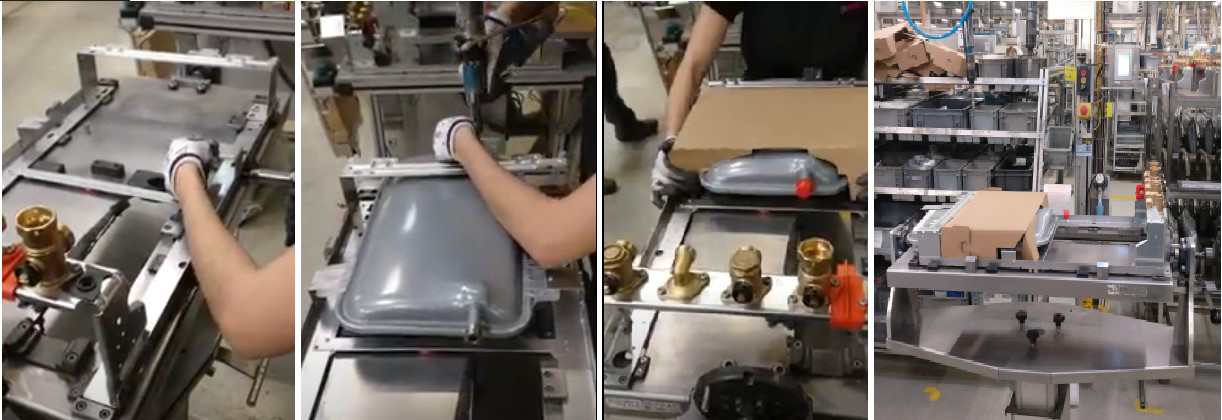
\includegraphics[width=6in]{figs/usecase.png}}
\caption{Different views of the current workstation used for the manual assemblage of the structure of a gas boiler for water heating.}
\label{fig:usecase}
\end{figure}

\section{Objectives}

The main objectives of this dissertation are:
\begin{itemize}
    \item Produce deep learning models capable of perceiving and recognizing the objects being grasped by the user by using the hand keypoints.
    
    \item Study the current research direction of Action Anticipation in the context of \acl{hrc} including common machine learning methods and how they impact the behavior of the robot.

    \item Develop an infrastructure to support a practical implementation of action anticipation in the context of the collaborative task and validate it with more simple experiments.

    \if{0}
    \item \textbf{Overview of the Experimental Setup}. Familiarization with the robot and tools that will be used throughout the dissertation.

    \item \textbf{Development of Action Anticipation Models}. To formally define how to anticipate an action in the context of the collaborative task under study using RGB-D images as input. \acs{ml} models, such as \acfp{rnn}, are at the forefront of the algorithms to explore.
    
    \item \textbf{Development of an Anticipatory Controller}. To develop robot controllers that consider the human partner's movements and intentions and use these inferences to make appropriate decisions during the execution of a sequential assembly task.

    \item \textbf{Metrics and performance evaluation}. To provide performance metrics used to evaluate the action anticipation models and the add-value of the anticipatory controller (e.g., in terms of cycle time).
    
    \item \textbf{Thesis Writing}. Writing the master dissertation and other detailed documentation.
    \fi
\end{itemize}

\section{Document Structure}

The remainder of the document is organized into four chapters. \textcolor{red}{Chapter \ref{chapter:state_of_the_art} contains background material about anticipation, \acl{ml} and collaborative robotics and a review of previous work on Action Anticipation in \acs{hrc} including sensors and methods. Chapter \ref{chapter:hrc_system} reviews tools that can be useful in the future implementation and ... Chapter \ref{chapter:learning} ... Chapter \ref{chapter:conclusion} concludes the document by restating the objectives of the work and...}
